\begin{figure}[t]
\centering
\subfigure[\gls{SLIC}]{%
  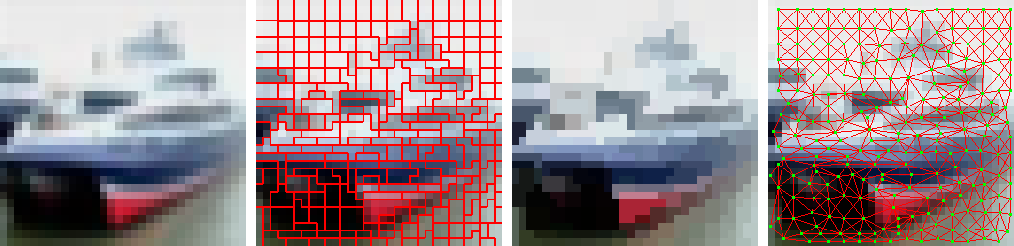
\includegraphics[width=\textwidth]{bilder/cifar_10_slic.png}
}
\subfigure[Quickshift]{%
  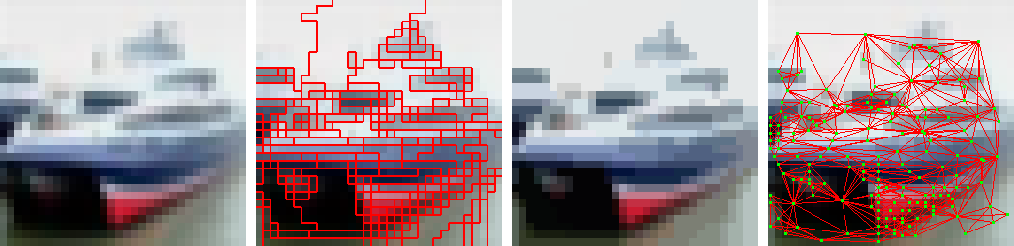
\includegraphics[width=\textwidth]{bilder/cifar_10_quickshift.png}
}
  \caption[\gls{Cifar}-10]{Bild aus dem \gls{Cifar}-10 Datensatz, jeweils dargestellt als (1) Originalbild, (2) Superpixelrepräsentation, (3) Durchschnittsfarbe der Superpixel und (4) Graphrepräsentation.}
\label{fig:cifar_10}
\end{figure}
